\documentclass[a4paper,12pt]{article}
\usepackage{amsmath}
\usepackage{amssymb}
\usepackage[utf8]{inputenc}
\usepackage[T1]{fontenc}
\usepackage{lmodern}
\usepackage{indentfirst}
\usepackage{geometry}
\usepackage{array}
\usepackage[pdftex]{color,graphicx}
\usepackage{subfigure}
\usepackage{afterpage}
\usepackage{setspace}
\usepackage{color}
\usepackage{wrapfig}
\usepackage{listings} 
\usepackage{datetime}
\usepackage{epstopdf}
\usepackage{hyperref}

\renewcommand{\onehalfspacing}{\setstretch{1.6}}

\geometry{tmargin=2.5cm,bmargin=2.5cm,lmargin=2.5cm,rmargin=2.5cm}
\setlength{\parindent}{1cm}
\setlength{\parskip}{0mm}

\newenvironment{lista}{
\begin{itemize}
  \setlength{\itemsep}{1pt}
  \setlength{\parskip}{0pt}
  \setlength{\parsep}{0pt}
}{\end{itemize}}

\newcommand{\linia}{\rule{\linewidth}{0.4mm}}

\definecolor{lbcolor}{rgb}{0.95,0.95,0.95}
\lstset{
  backgroundcolor=\color{lbcolor},
  tabsize=4,
  language=C++,
  captionpos=b,
  tabsize=3,
  frame=lines,
  numbers=left,
  numberstyle=\tiny,
  numbersep=5pt,
  breaklines=true,
  showstringspaces=false,
  basicstyle=\footnotesize,
  identifierstyle=\color{magenta},
  keywordstyle=\color[rgb]{0,0,1},
  commentstyle=\color{green},
  stringstyle=\color{red}
  }

\begin{document}

\noindent
\begin{tabular}{|c|p{11cm}|c|} \hline 
Michał Szczygieł & Aleksander Śmierciak & \ddmmyyyydate\today \tabularnewline
\hline 
\end{tabular}


\section*{Liczba PI metodą Monte Carlo w OMP}

Zadanie to polegało na zaimplementowaniu metody Monte Carlo, obliczającej przybliżoną wartośc liczby PI. Do zrównoleglenia obliczeń liczb pseudo losowych wykorzystany został interfejs OpenMP.
Metoda Monte Carlo użyta w tym programie opiera się na generowaniu losowych liczb z zakresu [0;1)

\begin{lstlisting}
unsigned int generatePoints(unsigned int threadCount, int pointCount)
{
	unsigned int wheelHits = 0;
	unsigned short seed[3];
	double x;
	double y;

	#pragma omp parallel num_threads(threadCount)
	{
		wheelHits = 0;
		initializeSeed(seed, threadCount);
		#pragma omp for firstprivate(seed) private(x,y) reduction(+:wheelHits)
		for (int i = 0; i < pointCount; i++)
		{
			x = erand48(seed);
			y = erand48(seed);
			if (std::pow(x, 2) + std::pow(y, 2) <= 1)
			{
				++wheelHits;
			}
		}
	}

	return wheelHits;
}
\end{lstlisting}

\textit{Czy w programie mozna zastosowac funkcje rand do otrzymywania liczb losowych? W jaki sposob zmodyfikowac dyrektywe OpenMP, aby była wydajniejsza niż domyślna? }
\\

Nie powinno się stosować funkcji rand() przy użyciu OpenMP, ponieważ funkcja ta nie jest zrównoleglana. Instrukcja rand() modyfikuje wewnętrzny stan generatora liczb pseudolosowych, możemy mieć do czynienia ze zjawiskiem wyścigu przy jej stosowaniu. Co więcej, modyfikacja globalnych obiektów wiąże się z zaburzeniami przetwarzania równoległego, co odbija się na zwiększającym się wraz ze zwiekszaniem liczby wątków czasie wykonania. 
Rozwiązaniami są alternatywne (dostarczane przez konkretne biblioteki) instrukcje, które bezpieczeństwo w architekturze wielowątkowej gwarantują, takie jak erand48().
\\
Dyrektywa OpenMP parallel for może zostać zastąpiona dyrektywą reduction.

\section*{Przebieg}
Obliczenia zostały wykonane na serwerze CUDA. Do zadania generowaliśmy 99999999 punktów. W każdym z przypadków uzyskano bardzo dobre przybliżenie liczby PI (z dokładnością do 6 miejsc po przecinku).\\



Poniżej wykresy przedstawiający rezultat przeprowadzonych operacji na wątkach.
\\
\begin{center}
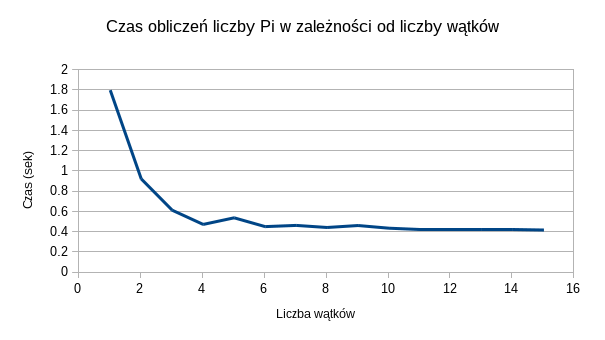
\includegraphics[width=0.7\textwidth]{data/przysp.png}
\end{center}


\begin{center}
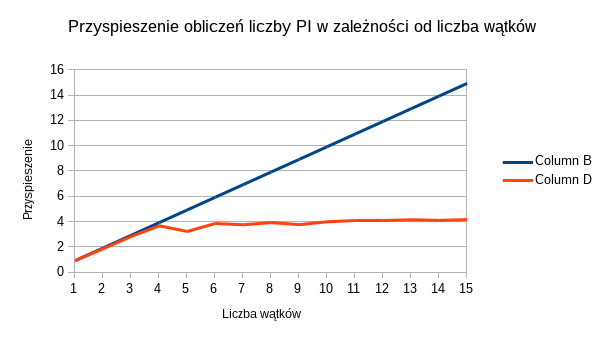
\includegraphics[width=0.7\textwidth]{data/speedup.png}
\end{center}


\section*{Wnioski}
Przy użyciu OpenMP możemy zrównoleglić każdy fragment kodu uzyskując przy tym wysoką wydajność na maszynach wielordzeniowych. Pomiary wykonywane na serwerze CUDA ilustują nam że przyspieszenie osiągane jest do 4 wątków. Gdyż wraz ze wzrostem liczby wątków obserwujemy spadek czasu potrzebnego na wykonanie programu. Ten spadek nie jest jednak liniowy - dla pewnej liczby wątków funkcja przyspieszenia stabilizuje się. Jest to związane z osiągnięciem stanu, w którym tworzenie kolejnych wątków, ich synchronizacja i zarządzanie są operacjami o kosztach przewyższających zyski ze zrównoleglania wykonywanych obliczeń.

\end{document}